\documentclass[]{article}
\usepackage{lmodern}
\usepackage{amssymb,amsmath}
\usepackage{ifxetex,ifluatex}
\usepackage{fixltx2e} % provides \textsubscript
\ifnum 0\ifxetex 1\fi\ifluatex 1\fi=0 % if pdftex
  \usepackage[T1]{fontenc}
  \usepackage[utf8]{inputenc}
\else % if luatex or xelatex
  \ifxetex
    \usepackage{mathspec}
  \else
    \usepackage{fontspec}
  \fi
  \defaultfontfeatures{Ligatures=TeX,Scale=MatchLowercase}
\fi
% use upquote if available, for straight quotes in verbatim environments
\IfFileExists{upquote.sty}{\usepackage{upquote}}{}
% use microtype if available
\IfFileExists{microtype.sty}{%
\usepackage{microtype}
\UseMicrotypeSet[protrusion]{basicmath} % disable protrusion for tt fonts
}{}
\usepackage[margin=1in]{geometry}
\usepackage{hyperref}
\hypersetup{unicode=true,
            pdftitle={R Installation},
            pdfauthor={Afra Humeid AlManei},
            pdfborder={0 0 0},
            breaklinks=true}
\urlstyle{same}  % don't use monospace font for urls
\usepackage{graphicx,grffile}
\makeatletter
\def\maxwidth{\ifdim\Gin@nat@width>\linewidth\linewidth\else\Gin@nat@width\fi}
\def\maxheight{\ifdim\Gin@nat@height>\textheight\textheight\else\Gin@nat@height\fi}
\makeatother
% Scale images if necessary, so that they will not overflow the page
% margins by default, and it is still possible to overwrite the defaults
% using explicit options in \includegraphics[width, height, ...]{}
\setkeys{Gin}{width=\maxwidth,height=\maxheight,keepaspectratio}
\IfFileExists{parskip.sty}{%
\usepackage{parskip}
}{% else
\setlength{\parindent}{0pt}
\setlength{\parskip}{6pt plus 2pt minus 1pt}
}
\setlength{\emergencystretch}{3em}  % prevent overfull lines
\providecommand{\tightlist}{%
  \setlength{\itemsep}{0pt}\setlength{\parskip}{0pt}}
\setcounter{secnumdepth}{0}
% Redefines (sub)paragraphs to behave more like sections
\ifx\paragraph\undefined\else
\let\oldparagraph\paragraph
\renewcommand{\paragraph}[1]{\oldparagraph{#1}\mbox{}}
\fi
\ifx\subparagraph\undefined\else
\let\oldsubparagraph\subparagraph
\renewcommand{\subparagraph}[1]{\oldsubparagraph{#1}\mbox{}}
\fi

%%% Use protect on footnotes to avoid problems with footnotes in titles
\let\rmarkdownfootnote\footnote%
\def\footnote{\protect\rmarkdownfootnote}

%%% Change title format to be more compact
\usepackage{titling}

% Create subtitle command for use in maketitle
\newcommand{\subtitle}[1]{
  \posttitle{
    \begin{center}\large#1\end{center}
    }
}

\setlength{\droptitle}{-2em}

  \title{R Installation}
    \pretitle{\vspace{\droptitle}\centering\huge}
  \posttitle{\par}
    \author{Afra Humeid AlManei}
    \preauthor{\centering\large\emph}
  \postauthor{\par}
      \predate{\centering\large\emph}
  \postdate{\par}
    \date{September 13, 2020}


\begin{document}
\maketitle

\hypertarget{main-programs}{%
\section{\texorpdfstring{\color{blue} Main
Programs}{ Main Programs}}\label{main-programs}}

For easily coding by R programming language you will need two main
programs:

\begin{enumerate}
\def\labelenumi{\arabic{enumi}.}
\tightlist
\item
  R
  
\includegraphics[width=0.15in,height=\textheight]{C:/Users/Afra/Dropbox/R programing/Install R/r.png}.
\item
  RStudio
  
\includegraphics[width=0.3in,height=\textheight]{C:/Users/Afra/Dropbox/R programing/Install R/rstudio.png}.
\end{enumerate}

The two programs are both free and available in the internet. First, you
will need to download the R program and install it. Then, download the
Rstudio and install it. Here, we will explain how to download and
install the two programs in details.

\hypertarget{how-to-download-and-install-r-program}{%
\subsection{\texorpdfstring{\color{blue} How to download and install R
program?}{ How to download and install R program?}}\label{how-to-download-and-install-r-program}}

\begin{enumerate}
\def\labelenumi{\arabic{enumi}.}
\tightlist
\item
  First go to the page \url{https://cran.r-project.org/}.
\item
  Press on the link that has the same as your computer operating system
  (OS). See the picture bellow.
\end{enumerate}

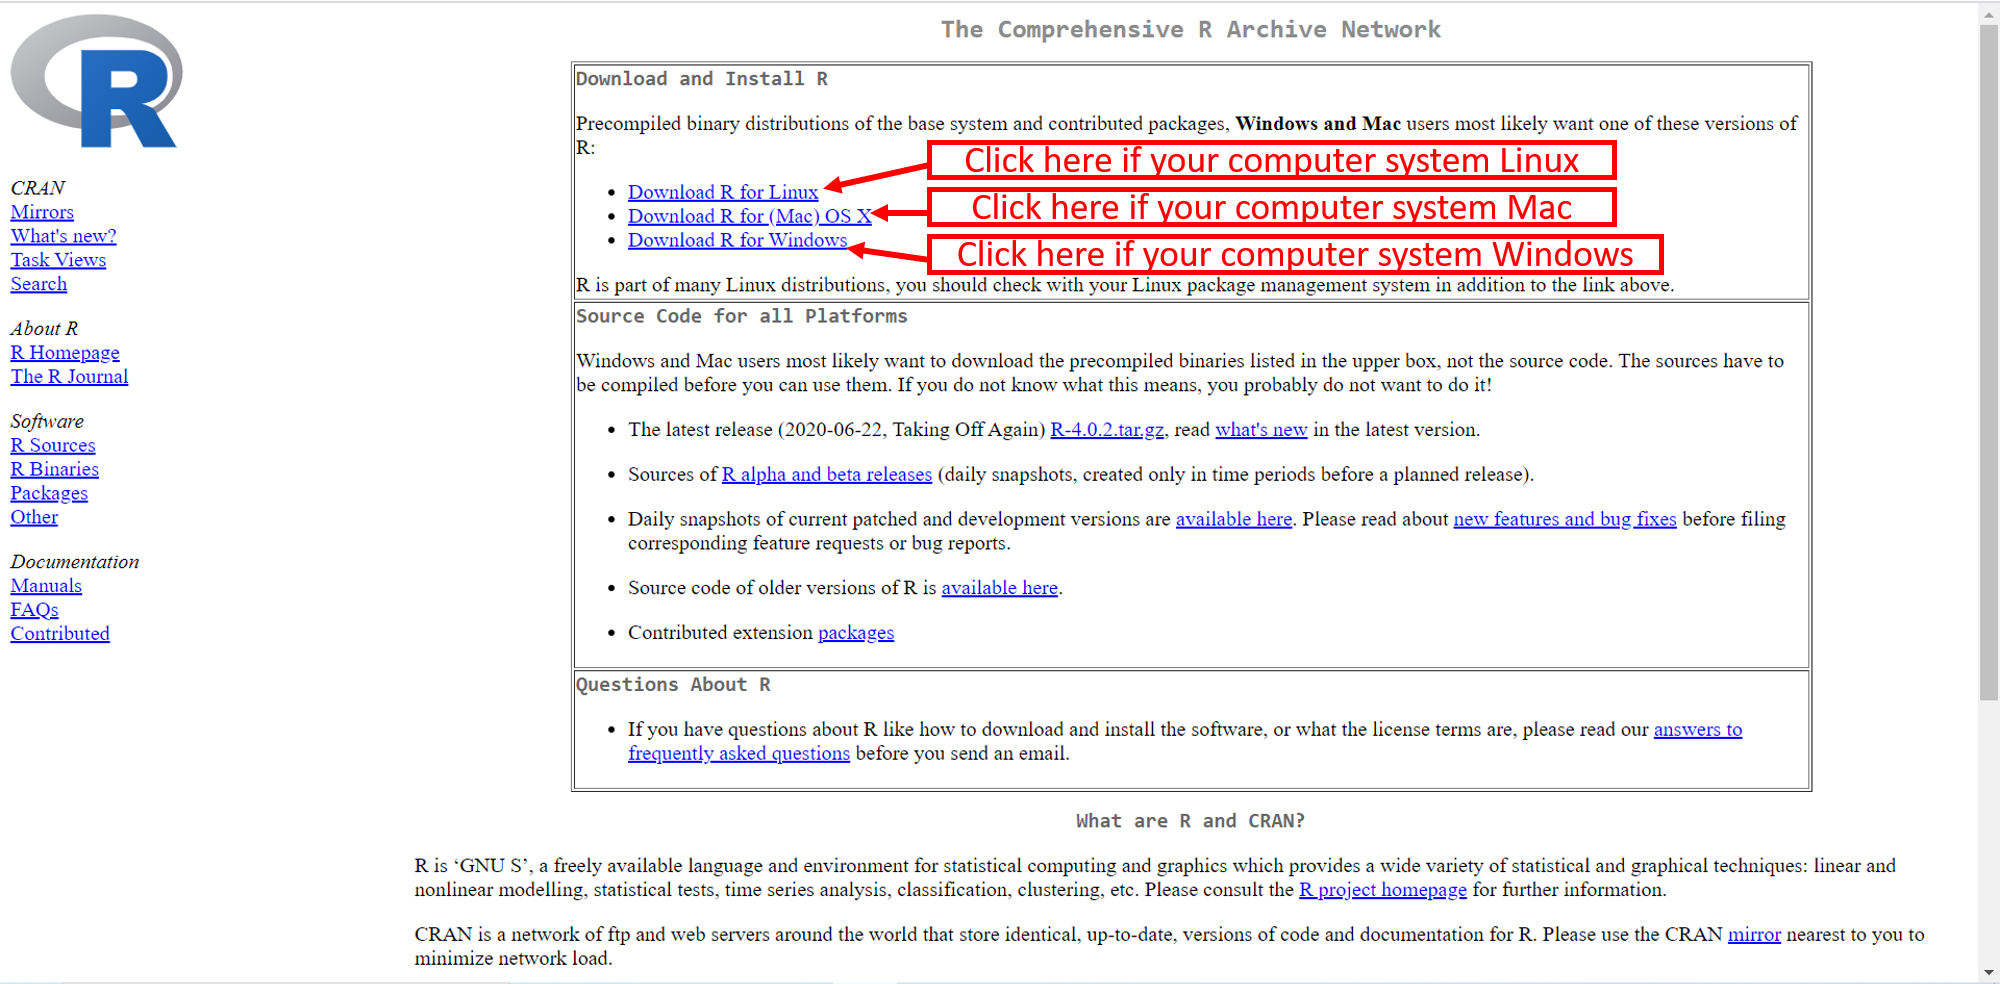
\includegraphics[width=1\linewidth]{C:/Users/Afra/Dropbox/R programing/Install R/step1}

\hypertarget{for-windows}{%
\subsubsection{\texorpdfstring{\color{blue} For
Windows}{ For Windows}}\label{for-windows}}

For Windows the next step is to press on the \textbf{install R for the
first time} as shown in the picture bellow.

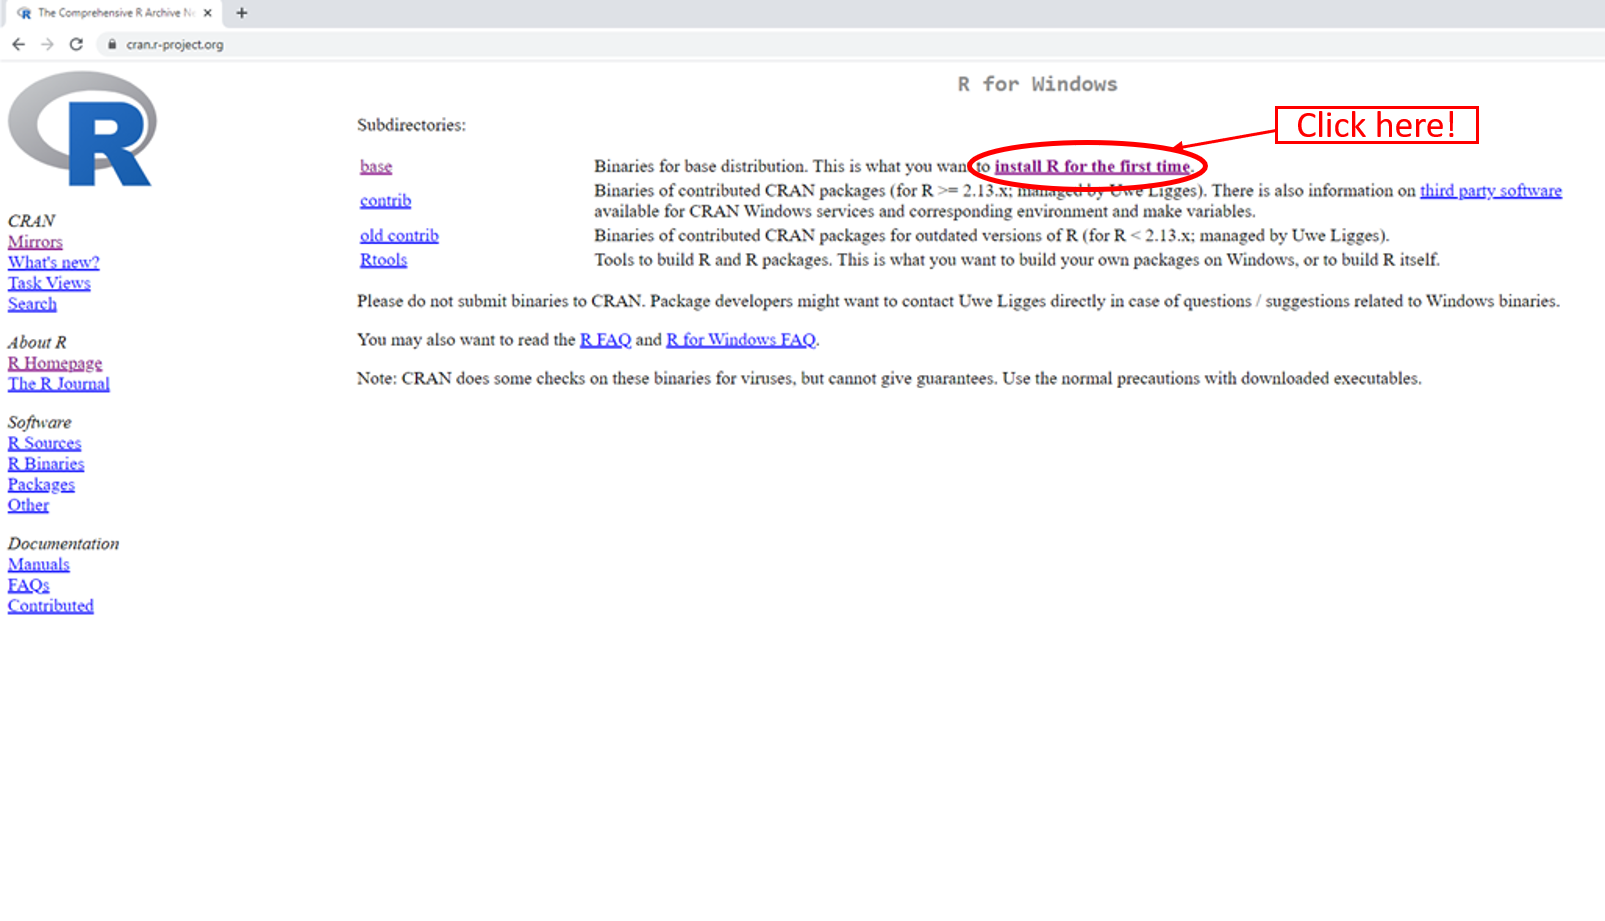
\includegraphics[width=1\linewidth]{C:/Users/Afra/Dropbox/R programing/Install R/step2windows}

Then, you press on \textbf{Download R 4.0.2 for Windows} as shown in the
picture bellow.

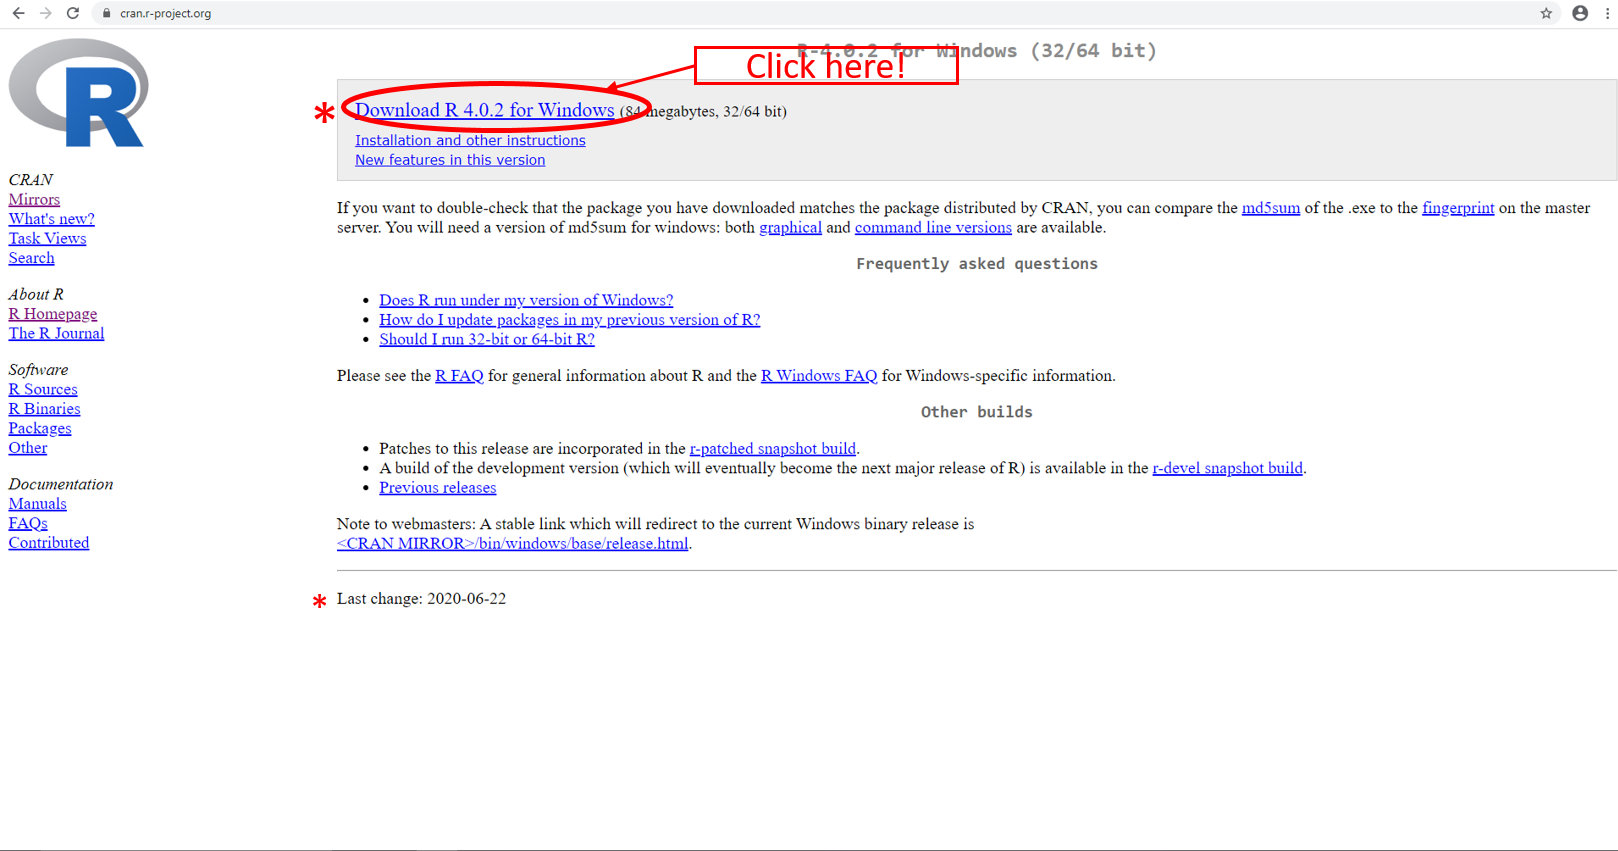
\includegraphics[width=1\linewidth]{C:/Users/Afra/Dropbox/R programing/Install R/step3windows}

Then, the \textbf{R} program will be downloaded. Once finish the
download, you go to the file that you have downloaded and click on it
and select \textbf{Open}. Then, follow the instructions in the pictures
bellow.

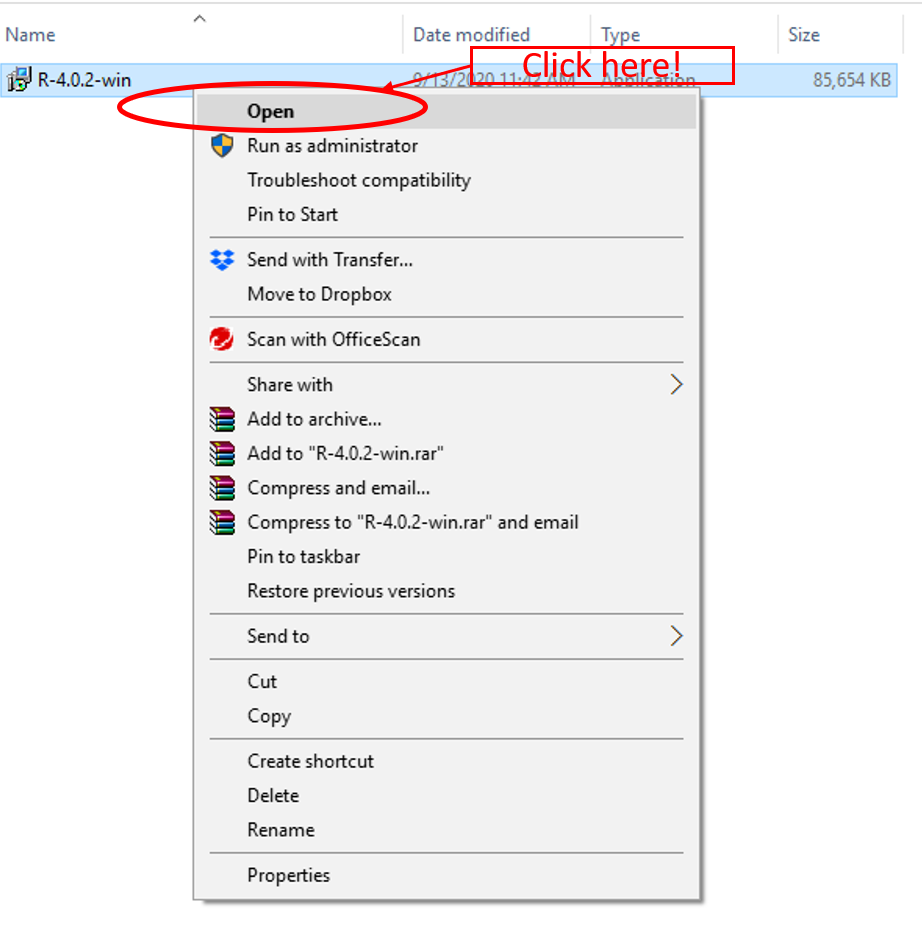
\includegraphics[width=1\linewidth]{C:/Users/Afra/Dropbox/R programing/Install R/step4windows}

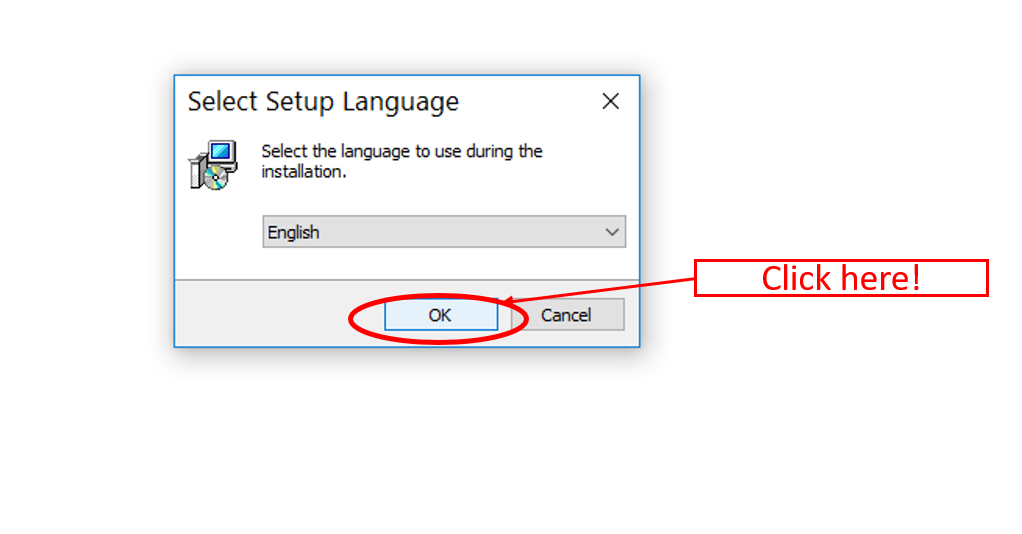
\includegraphics[width=1\linewidth]{C:/Users/Afra/Dropbox/R programing/Install R/step5windows}

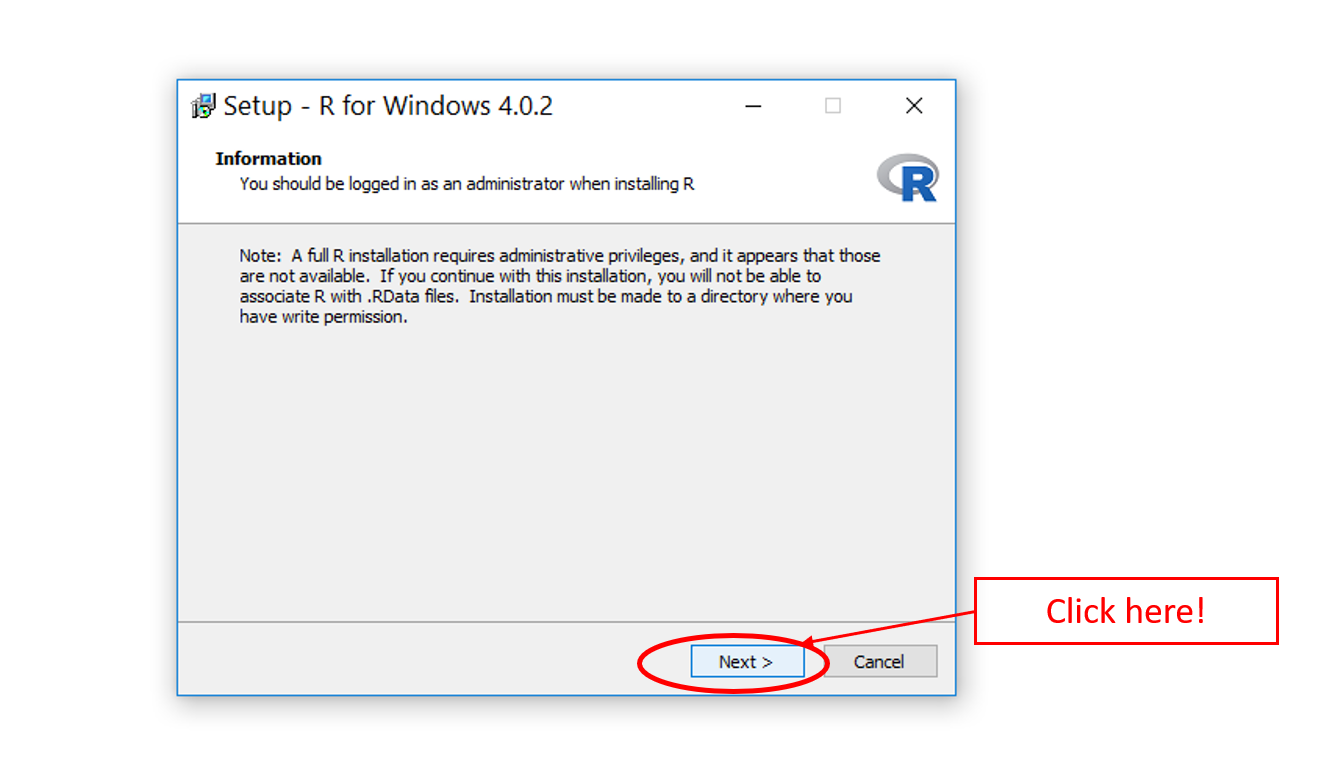
\includegraphics[width=1\linewidth]{C:/Users/Afra/Dropbox/R programing/Install R/step6windows}

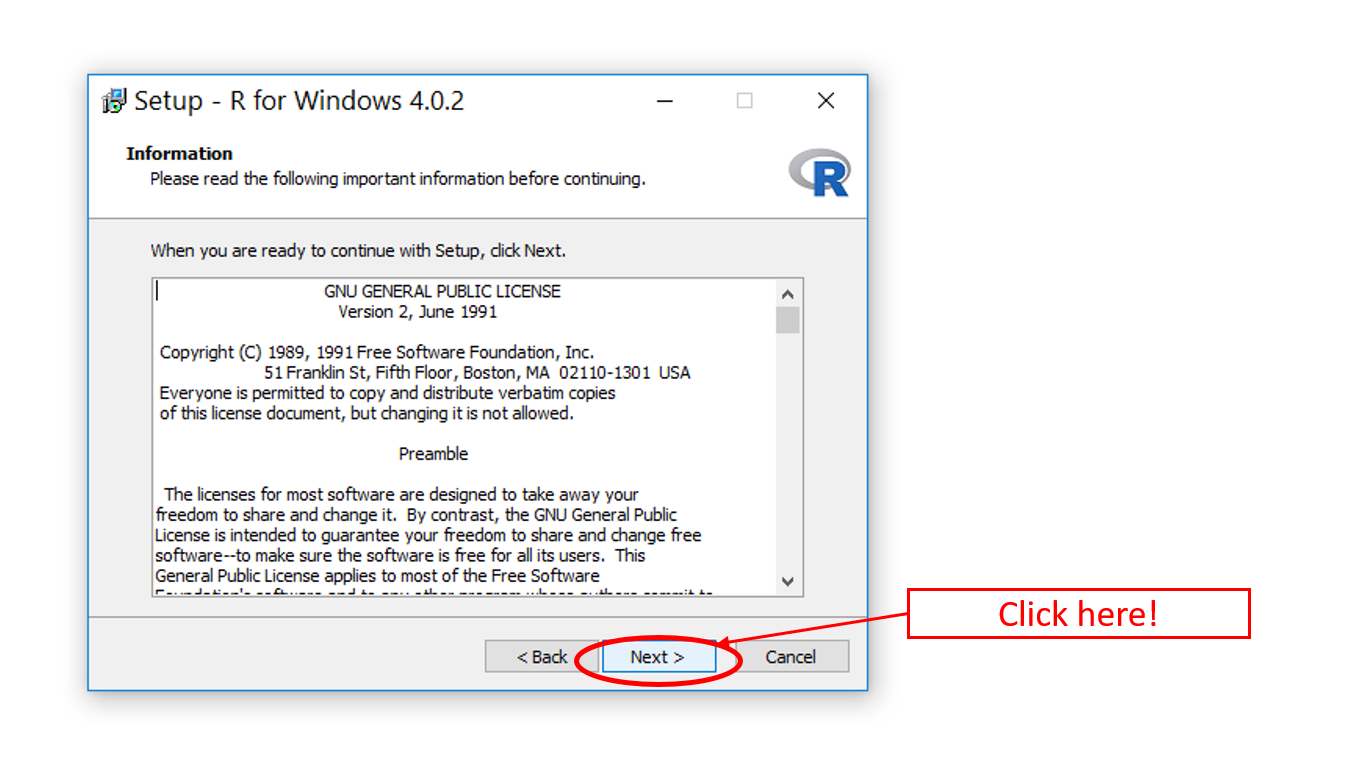
\includegraphics[width=1\linewidth]{C:/Users/Afra/Dropbox/R programing/Install R/step7windows}

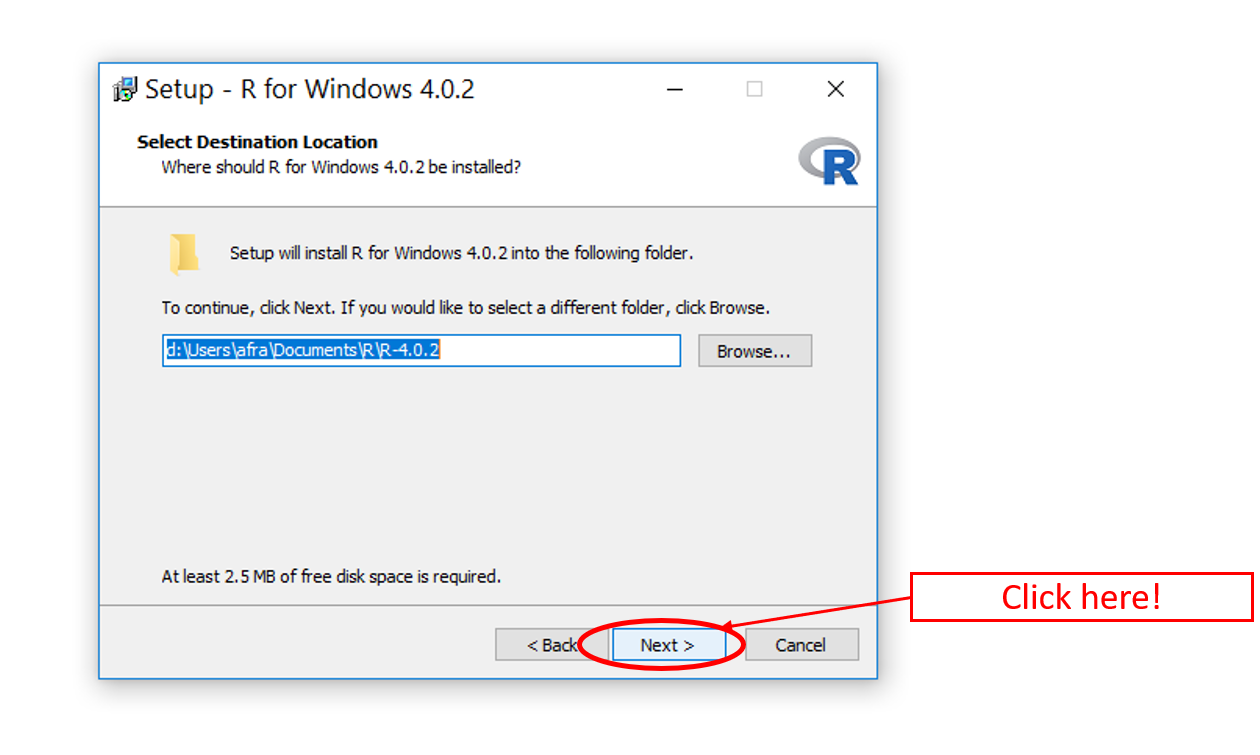
\includegraphics[width=1\linewidth]{C:/Users/Afra/Dropbox/R programing/Install R/step8windows}

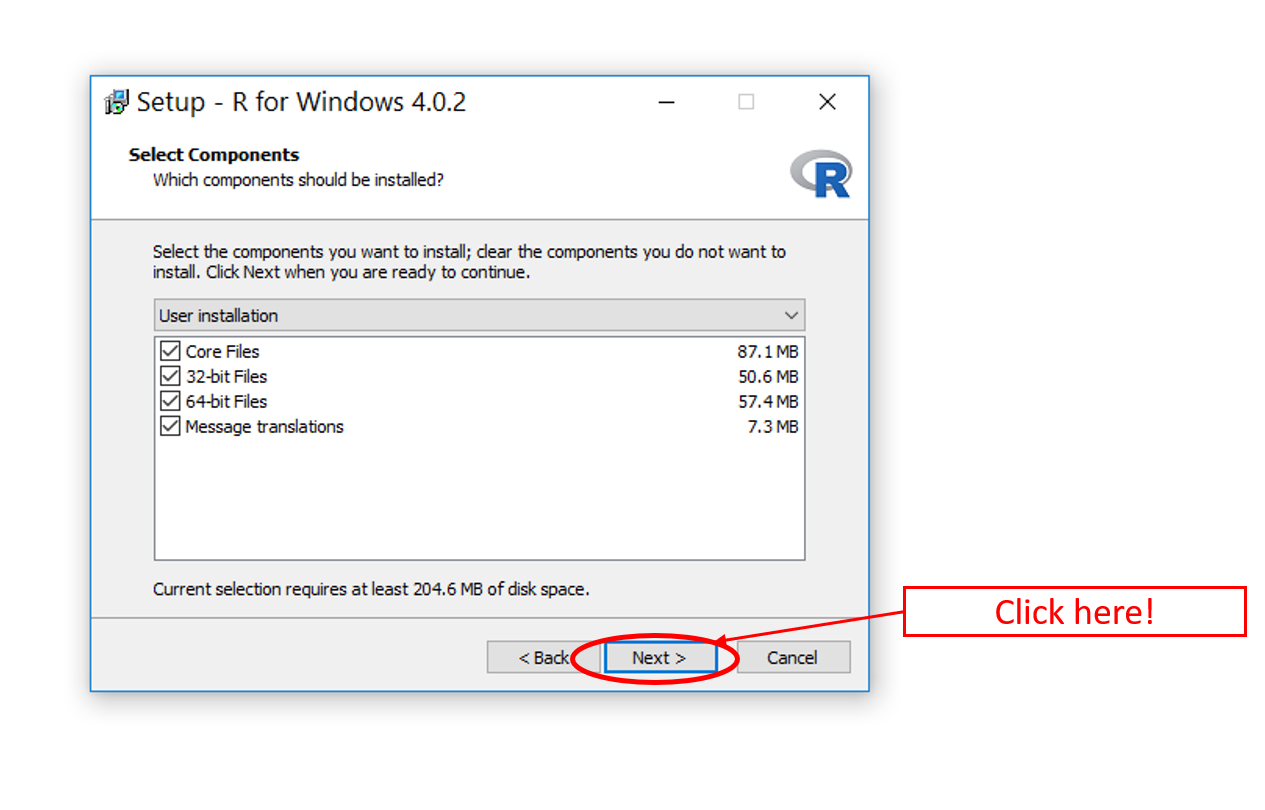
\includegraphics[width=1\linewidth]{C:/Users/Afra/Dropbox/R programing/Install R/step9windows}

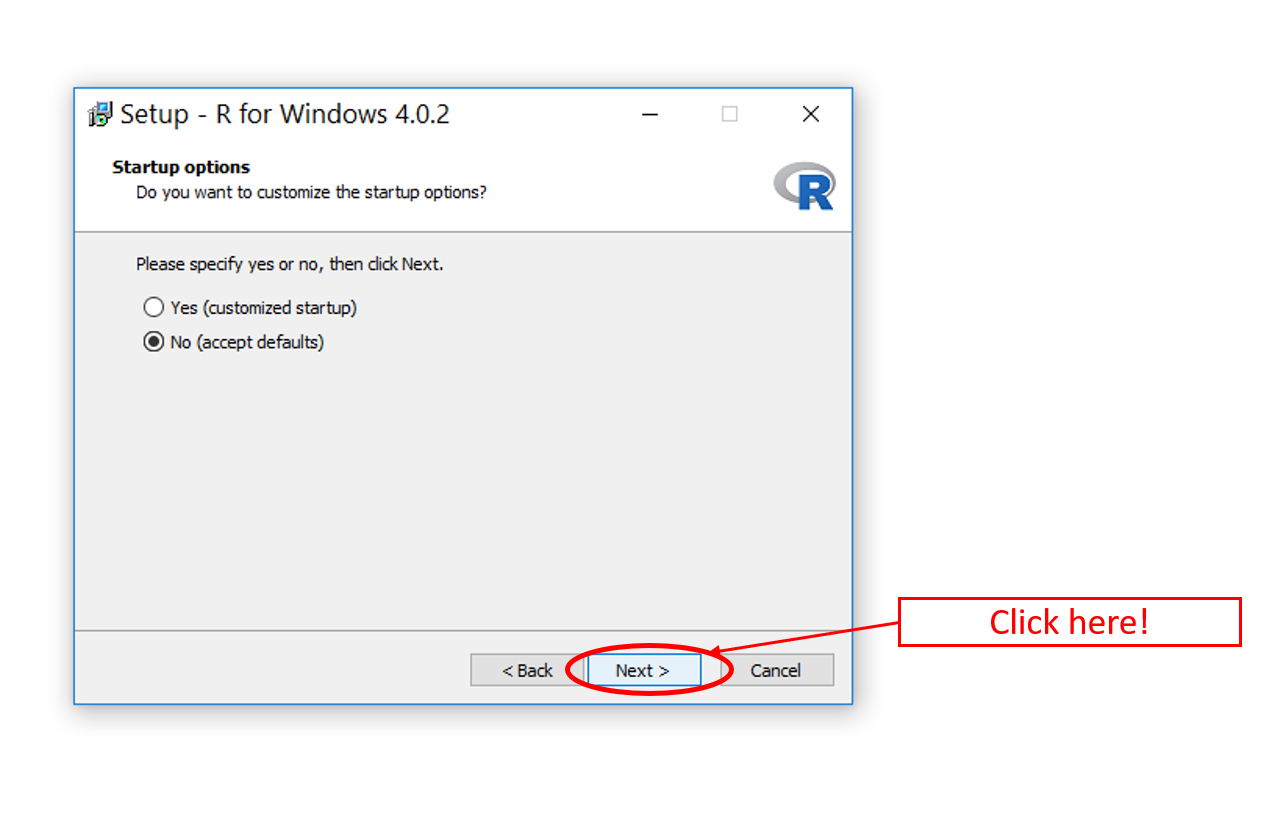
\includegraphics[width=1\linewidth]{C:/Users/Afra/Dropbox/R programing/Install R/step10windows}

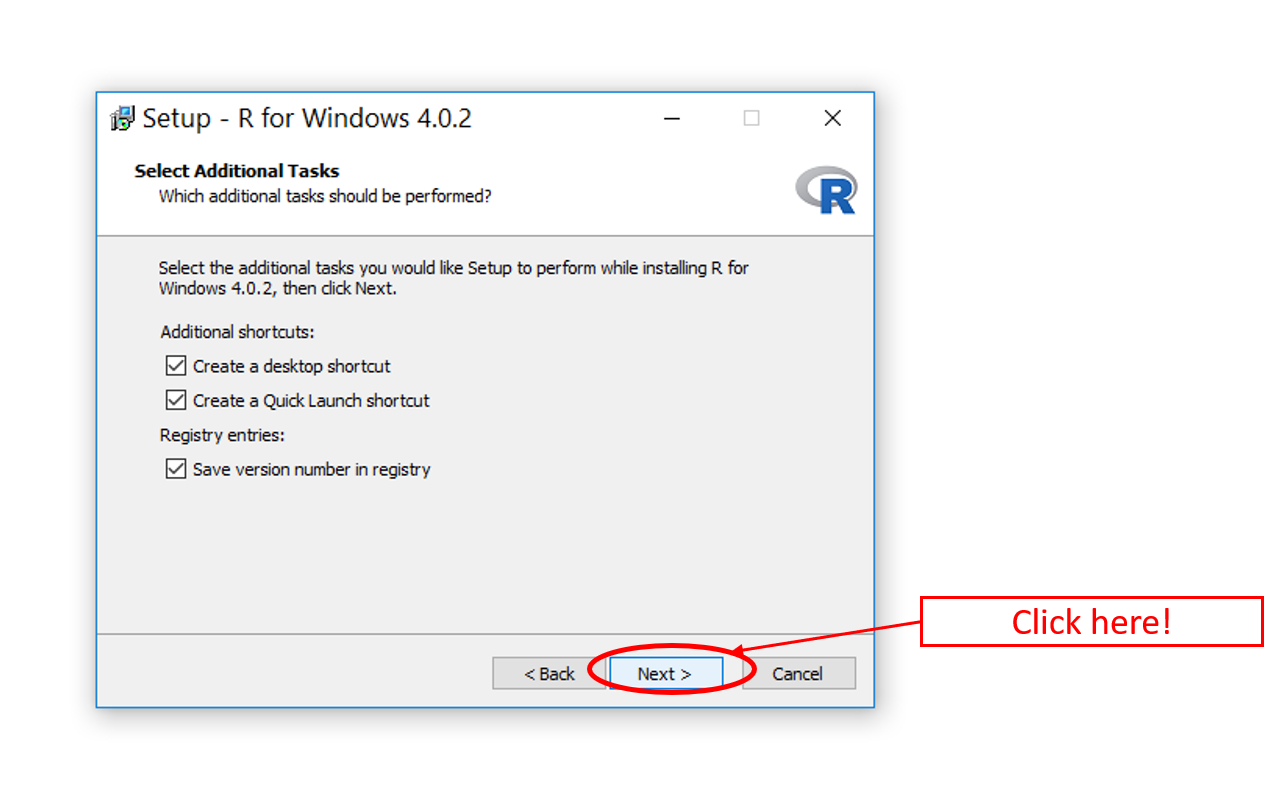
\includegraphics[width=1\linewidth]{C:/Users/Afra/Dropbox/R programing/Install R/step11windows}

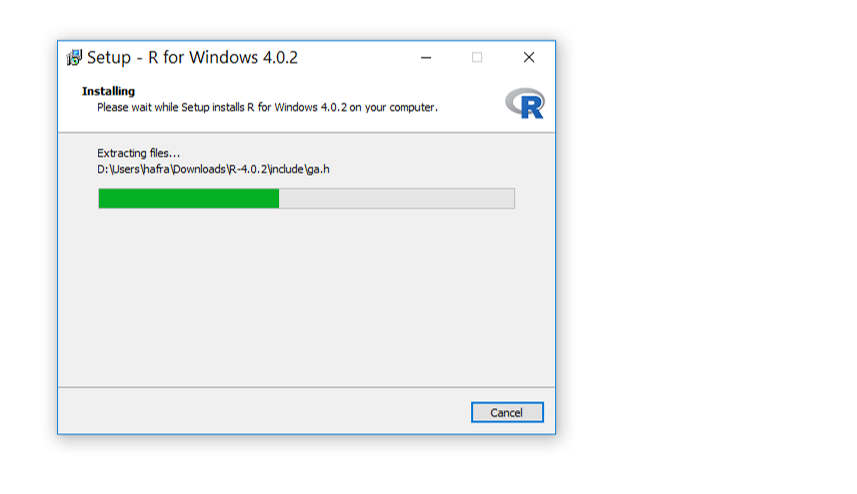
\includegraphics[width=1\linewidth]{C:/Users/Afra/Dropbox/R programing/Install R/step12windows}

Now, the \textbf{R} program is in your computer.


\end{document}
